\chapter{Civilingenjörsutbildning i Mjukvaruteknik}

\begin{tcbdoublebox}
\emph{Avsnittet täcker aspekten Yrkesexamen i den föreslagna ansökningsmallen. Här anges vilken examen som anses och när programstart kommer att ske. En analys av utbildningens omfattning och innehåll i förhållande till den vetenskapliga grunden samt dess vetenskapliga bredd och djup finns också med.}
\end{tcbdoublebox}

Denna ansökan gäller examenstillstånd för \emph{civilingenjör med en inriktning mot mjukvaruteknik}. Den engelska examensbenämningen är \emph{Degree of Master of Science in Engineering, Software Technology}.

Den föreslagna civilingenjörsutbildningen fokuserar på processer, metoder och tekniker för utveckling av mjukvara

som utgör en del av större system. Utbildningen har sin huvudsakliga ämnesbas i datavetenskap (Computer Science enligt ACM:s nomenklatur\footnote{Association for Computing Machinery~(ACM) (\url{https://www.acm.org}), förening för vetenskap och utbildning inom området datavetenskap.}) och mjukvaruutveckling (Software Engineering enligt samma nomenklatur). Dessa utgör programmets karaktärsämnen. Eftersom det finns en stark koppling mellan datavetenskap och matematik har utbildningen även en del av sin ämnesbas där. Mjukvaruutveckling sker i projekt och i team varför förmåga att kommunicera, både på svenska och på engelska, samt att arbeta i grupp är avgörande för att studenten ska fungera i sin framtida yrkesroll. Tillsammans med exempelvis elektroteknik och fysik utgör dessa programmets kärnämnen.

En utexaminerad civilingenjör förväntas efter en tid kunna gå in i samtliga utvecklingsrelaterade roller i ett mjukvaruutvecklingsprojekt, från teknisk expert till projektledare. Utbildningen ger också en bra grund för att starta och driva egen verksamhet samt för en akademisk karriär med forskning och utbildning inom datavetenskap.

Den föreslagna civilingenjörsutbildningen kommer att ges på helfart och vara förlagd till Campus Växjö. Starten på utbildningen planeras till höstterminen 2020. Det skapar ett tillräckligt utrymme för nödvändiga förberedelser inför utbildningsaktiviteterna samt marknadsföring av utbildningen. Utbildningen planeras till en början för 35 studenter per år. Antalet är valt för att säkra kvaliteten i utbildningen och att det initialt finns tillräckligt med handledarresurser för projekt och självständiga arbeten.


\section{Utbildningens struktur och innehåll}

\begin{table}[t]
\centering
\caption{Fördelning av högskolepoäng på huvudämnen i utbildningen.\label{tab:poangf}}
\begin{threeparttable}
\begin{tabular}{lrr}
\toprule
\textbf{\textsf{Huvudämne}} & \textbf{\textsf{Obligatoriska}} & \textbf{\textsf{Valbara}} \tabularnewline
\midrule
Datavetenskap & 190 & 15 \tabularnewline
Matematik & 45 & 5\tabularnewline
Fysik & 15 & \tabularnewline
Elektroteknik\tnote{1} & 5 & \tabularnewline
Teknik-Människa-Samhälle\tnote{2,3} & 20 & 5 \tabularnewline
\bottomrule
\end{tabular}
\begin{tablenotes}
\item[1] Reglerteknik
\item[2] Huvudämnet Teknik-Människa-Samhälle används enbart för att förenkla uppställningen.
\item[3] Grundkurs i vetenskapliga metoder räknas som Teknik-Människa-Samhälle, fortsättningskurs är inom ämnet.
\end{tablenotes}
\end{threeparttable}
\end{table}

Den föreslagna utbildningen omfattar 300 högskolepoäng (hp). Poängen är fördelade enligt tabell~\ref{tab:poangf}. Av de 300 hp är 25 hp valbara kurser som ger studenterna möjlighet att bredda eller fördjupa sig. För varje valbar kurs finns en rekommenderad fördjupande kurs, av dessa är 20 hp datavetenskap och 5 hp matematik. De 190 hp datavetenskap innehåller 32,5 hp projektkurser och två självständiga arbeten, om 15 respektive 30 hp.

Utbildningen är uppbyggd som en sammanhållen 5-årig utbildning som omfattar de två första cyklerna enligt Bolognaprocessen: grund- och avancerad nivå. Årskurs 1–3 av utbildningen ger grundläggande kunskaper i kärn- och karaktärsämnen och årskurs 4–5 ger en fördjupning inom karaktärsämnen kopplade till forskningsområden inom datavetenskap. Detta upplägg är inspirerat av utbildningar på Kungliga Tekniska Högskolan\footfullcite{rosen2011} och en liknande struktur återfinns vid andra lärosäten såsom Chalmers Tekniska Högskola.

De två följande avsnitten beskriver innehåll och progression i delarna på grund och avancerade nivå. Utbildningsplan för hela utbildningen bifogas i appendix~\ref{app:utbplan} och samtliga kursplaner bifogas i appendix~\ref{app:kursplaner}.

\subsection{Utbildningens innehåll och progression årskurs 1--3}

\begin{figure}[t]
\centering
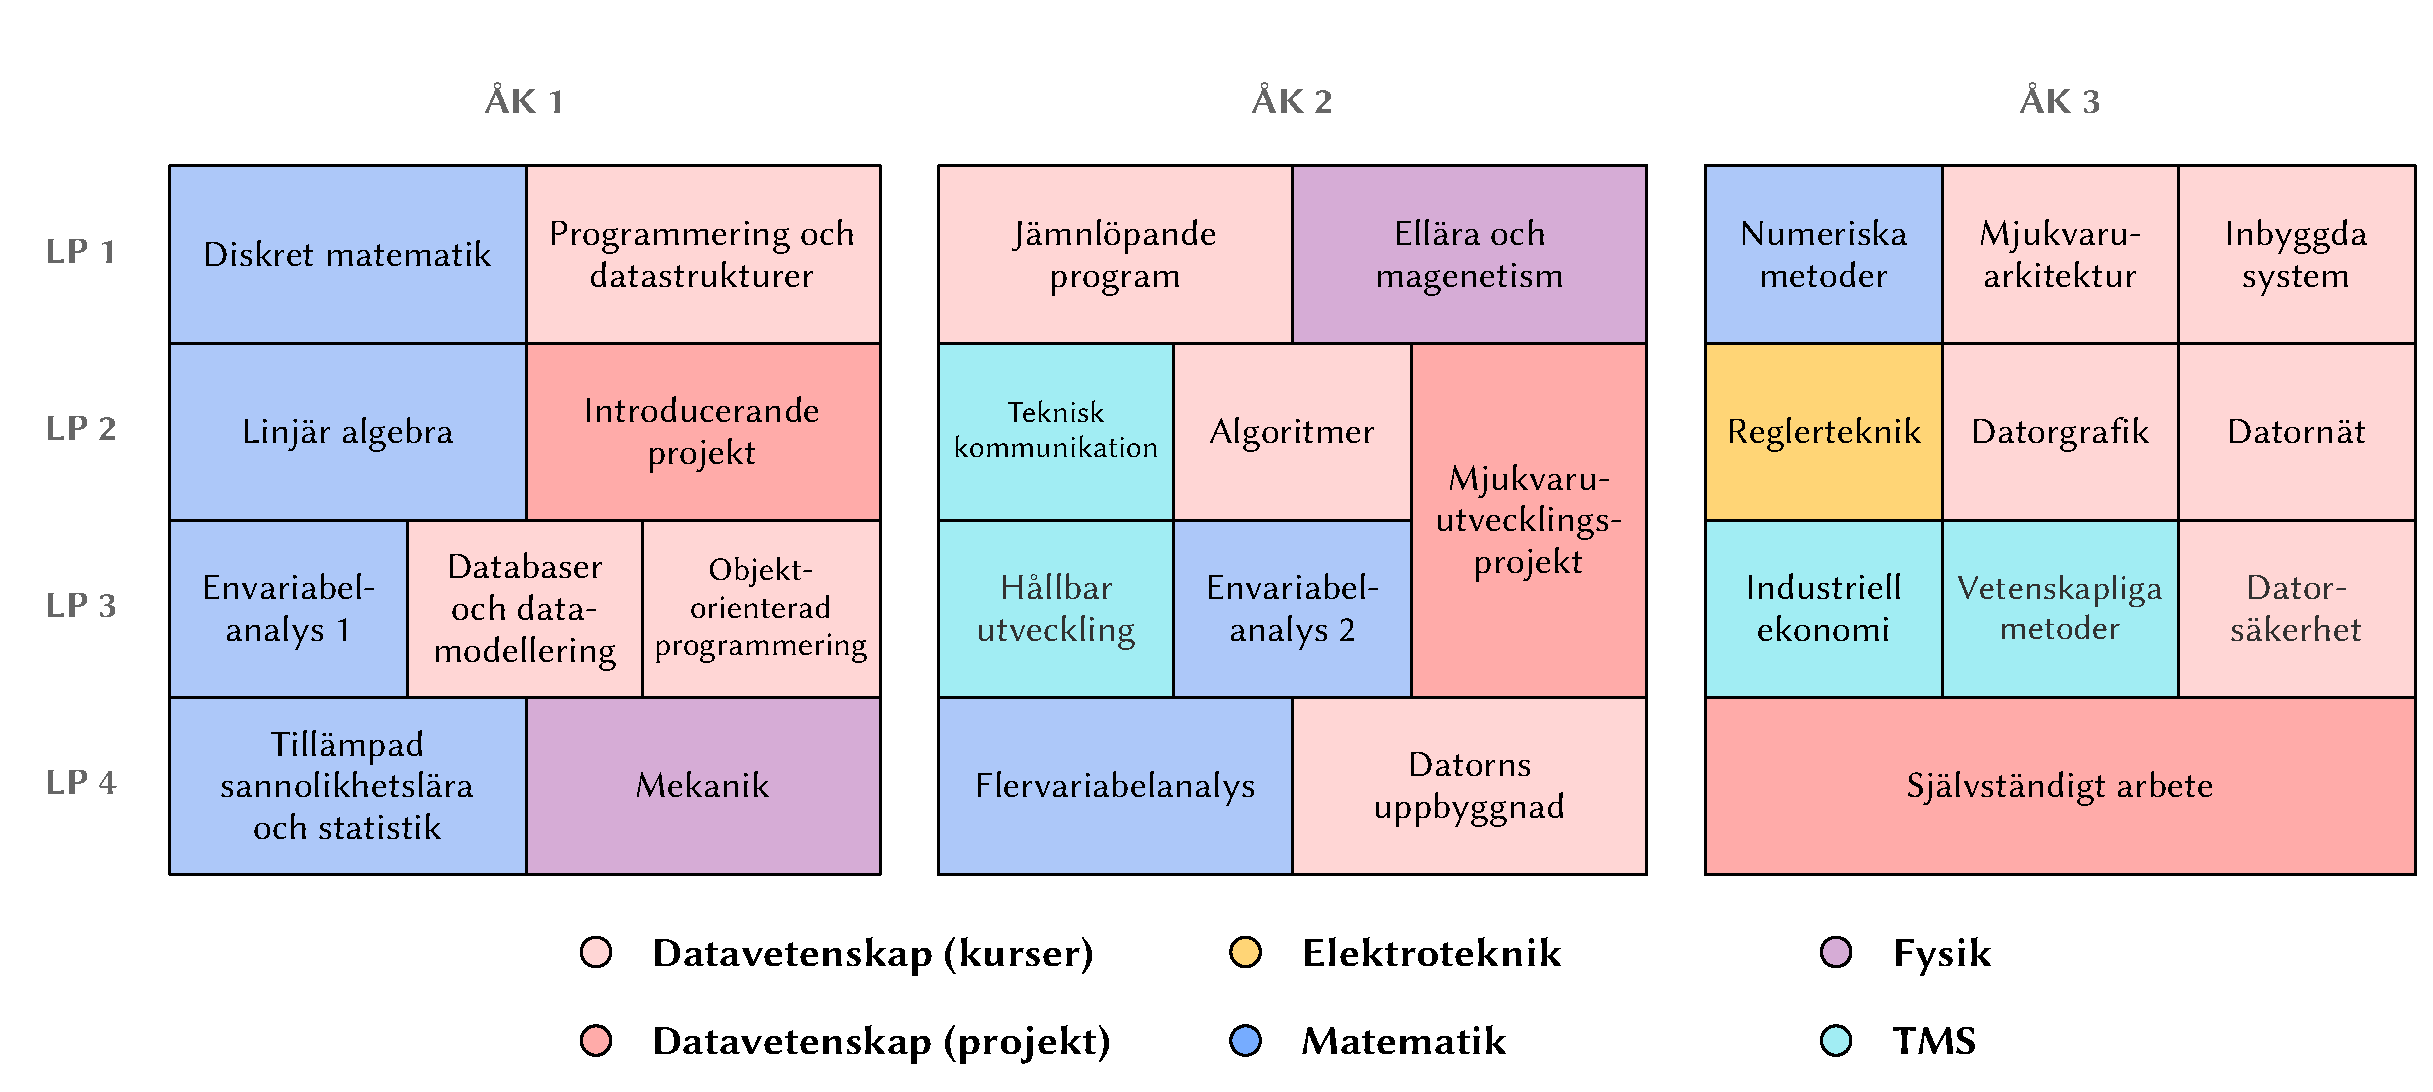
\includegraphics[width=\columnwidth]{images/bs13.eps}
\caption{Upplägg årskurs 1--3. Varje läsperiod omfattar 15 hp och kurserna omfattar 5, 7,5 eller 10 hp. Det självständiga arbetet omfattar 15 hp.\label{fig:bs13}}
\end{figure}

Årskurs 1--3 motsvarar innehållsmässigt en kandidatutbildning inom datavetenskap med särskilt fokus på yrkesmässighet och teknik, människa och samhälle. Figur~\ref{fig:bs13} beskriver innehåll och progression under årskurs 1--3. Det datavetenskapliga innehållet är upplagt enligt ACM och IEEE:s\footnote{Institute of Electrical and Electronics Engineers~(IEEE) (\url{https://www.ieee.org}), en internationell branchorganisation för ingenjörer inom elektroteknik, telekommunikation, och datateknik.} gemensamma rekommendationer för innehåll i utbildning på grundnivå (ACM CS2013)\footfullcite{cs2013}. Conceive-Design-Implement-Operate (CDIO)-konceptett\footfullcite{crawley2014rethinking} används för att säkerställa att utbildningen och dess kurser innehåller en hög nivå av ingenjörsmässighet. Innehållet i kurserna i matematik och fysik är valt för att ge en tillräcklig grund inom dessa ämnen samt stödja kurser i karaktärsämnet.

Då upplägget och kurserna bygger på ACM CS2013 påminner blockschemat om flera andra grundutbildningar inom datavetenskap vid Linnéuniversitetet. Under arbetet med det föreslagna utbildningsprogrammet har stor vikt lagts vid progression och färdighetsbyggande. Innehållet i årskurs 4 och 5 definierades först och sedan planerades årskurs 1–3 så att de bygger upp de färdigheter och kunskaper som behövs. Resterande delen av avsnittet fokuserar på de huvudsakliga progressionsspåren.

Det finns ett starkt samspel mellan datavetenskap och matematik, men detta är av erfarenhet svårt att kommunicera till studenterna. Det föreslagna programmet skapar därför tydliga kopplingar mellan kurserna i datavetenskap och matematik under årskurs 1. Under läsperiod 1 får studenterna se datastrukturer från ett datavetenskapligt perspektiv i \emph{Programmering och datastrukturer} och från ett matematiskt perspektiv i \emph{Diskret matematik}. Den senare innehåller inte någon undervisning i programmering, men kommer att ha frivilliga programmeringsuppgifter som studenterna kan göra för att utforska likheterna och för att ta sig an matematiken från ett datavetenskapligt perspektiv. I läsperiod 2 presenteras programmering i Matlab i kursen \emph{Linjär algebra} och studenterna kan direkt tillämpa färdigheter från datavetenskap. På liknande sätt tillämpas begrepp från matematiken, exempelvis funktionsbegreppet och matematisk logik, i kursen \emph{Databaser och datamodellering} i läsperiod 3. I övriga kurser i datavetenskap och matematik använder, när tillämpbart, exempel från det andra ämnet, det vill säga datavetenskapliga tillämpningar inom kurserna i matematik och matematiska problem i kurserna i datavetenskap. I kursen \emph{Numeriska metoder} i läsperiod 1, årskurs 3 studeras bland annat numeriska grafalgoritmer och Bézier-kurvor, som båda har flera tillämpningar inom datavetenskap.

Programmering är en grundläggande färdighet och utbildningen är byggd runt fyra programmeringsspråk: C, Java, Matlab och Python. En kurs kan, så länge den ges efter språket introducerats, välja att använda det av dessa som bäst lämpar sig för kursens innehåll eller låta studenterna välja fritt. Om en kurs behöver ett annat språk ingår det som lärandemål för kursen. Kursen \emph{Programmering och datastrukturer} lär ut grundläggande imperativ programmering och vissa koncept från funktionell programmering med hjälp av Python. Det föreslagna programmet börjar med ett programmeringsspråk som anses lätt att lära sig för att kunna lägga fokus på problemlösning och algoritmer. Kursen \emph{Objektorienterad programmering} bygger vidare på dessa färdigheter och lär ut objektorienterad programmering i Java medan kursen \emph{Datorns uppbyggnad} fokuserar på hårdvarunära programmering med C. Matlab ingår i kurserna i matematik och introduceras i kursen \emph{Linjär algebra}.

Vårt upplägg medför att studenterna får lära sig tre programmeringsspråk under årskurs 1. Detta upplägg har valts för att belysa att programmeringsspråket är ett verktyg och att olika språk är mera lämpliga än andra i vissa situationer. Vart och ett av språken kommer att användas i en rad kurser under utbildningen och på så sätt fördjupa studentens förståelse för och färdighet i språket.

En annan grundläggande färdighet är modellering och tänkande i modeller. Detta börjar ur ett mjukvaruutvecklingsperspektiv i kurserna \emph{Databaser och datamodellering} och \emph{Objektorienterad programmering} i årskurs 1, där studenterna får två olika perspektiv på objektorienterad modellering samt en introduktion till problemlösning på modellnivå med designmönster. Studenterna tillämpar dessa färdigheter i kursen \emph{Mjukvaruutvecklingsprojekt} i årskurs 2 och de fördjupas i kursen \emph{Mjukvaruarkitekturer} i årskurs 3.

Yrkesfärdigheter och ingenjörsmässighet undervisas genom kurser i teknik, människa och samhälle samt en serie projektkurser. Studenterna introduceras till yrkesrollen mjukvaruingenjör redan i kursen \emph{Programmering och datastrukturer}, genom de verktyg som används och enklare samarbetsformer (exempelvis parprogrammering). Detta byggs vidare i kursen \emph{Introducerande projekt}, där studenterna ges insikt i yrkesrollen genom bland annat gästföreläsningar och studiebesök. Projektarbetet sker under enkla men realistiska förhållande och täcker hela Concieve-Design-Implement-Operate-cykeln från CDIO-konceptet. Det ger på så sätt ytterligare insikt i de verktyg och arbetssätt som används och vikten av att förstå vilket problem ett mjukvarusystem skall lösa.

I årskurs 2 fångas erfarenheterna från tidigare ämnes- och projektkurser upp i \emph{Teknisk kommunikation} och \emph{ållbar utveckling}. Den första av dessa belyser rapportskrivande och muntlig presentation. Den senare belyser hållbarhet ur sociala, miljömässiga och ekonomiska perspektiv. I kursen \emph{Introducerande projekt} reflekterar studenterna över yrkesrollen mjukvaruingenjör från ett personligt perspektiv. Efter denna introduktion kan ett socialt perspektiv läggas till genom att studenterna exempelvis inom ramen för inlämningsuppgifter reflekterar över den ojämna könsfördelningen inom mjukvaruindustrin och vilken påverkan den har i stort. Kursen \emph{Mjukvaruutvecklingsprojekt} fördjupar förståelse för yrkesrollen, dels genom ytterligare gästföreläsningar eller studiebesök, men främst genom en fördjupning i de verktyg och de arbetssätt som används. Kursen består av ett realistiskt projekt där studenterna löser ett problem åt en kund genom att tillämpa en agil mjukvaruutvecklingsprocess. Kursen \emph{Industriell ekonomi} i årskurs 3 belyser ekonomi ur ett industriellt perspektiv och påvisar skillnader och likheter mellan exempelvis traditionell tillverkningsindustri och mjukvaruindustrin, såsom utvecklings- kontra tillverkningskostnad. Ekonomi beskrivs också ur ett samhällsperspektiv där exempelvis mjukvarans ökande roll diskuteras och hur det kommer att påverka samhälle och industri.

Kurserna inom teknik, människa och samhälle har utformats och placerats så att det ämne som behandlas inom en kurs kan introduceras innan kursen ges och sedan kan byggas vidare på och fördjupas. Hållbarhet lyfts fram ur olika perspektiv under kurserna i årskurs 1 på en ytlig nivå (Introduceras, enligt CDIO-terminologi) och dessa perspektiv fångas upp och fördjupas inom kursen hållbar utveckling (Undervisas). I efterföljande kurser behandlas hållbarhetsperspektiven djupare och erfarenheter och teorier används direkt (Undervisas och Används).

Årskurs 3 avslutas med två kurser som samlar upp erfarenheter och perspektiv från tidigare kurser. Den första av dessa är kursen \emph{Datorsäkerhet}, som diskuterar erfarenheter från bland annat kurserna \emph{Databaser och datamodellering} och \emph{Datornät} och belyser dem ur ett säkerhetsperspektiv. Frågeställningar såsom vilka problem som finns, hur de kan lösas, samt hur man tänker kring säkra system diskuteras. Dessa perspektiv kommer, likt perspektiv från kurserna i teknik, människa och samhälle, tas med i framtida kurser och beröras där det är tillämpligt. Den andra sammanfattande kursen är det självständiga arbetet, där studenterna tillämpar kunskaper och färdigheter från årskurs 1–3 för att formulera och lösa ett problem, samt beskriva och argumentera för lösningen. Dessa färdigheter är viktiga och det föreslagna programmet innehåller därför ett självständigt arbete om 15 hp i slutet av årskurs 3, för att sammanfatta och förbereda studenterna inför studier på avancerad nivå, där den vetenskapliga kopplingen och kraven på bland annat rapporter skärps.

\subsection{Utbildningens innehåll och progression årskurs 4--5}

\begin{figure}[tbp]
\centering
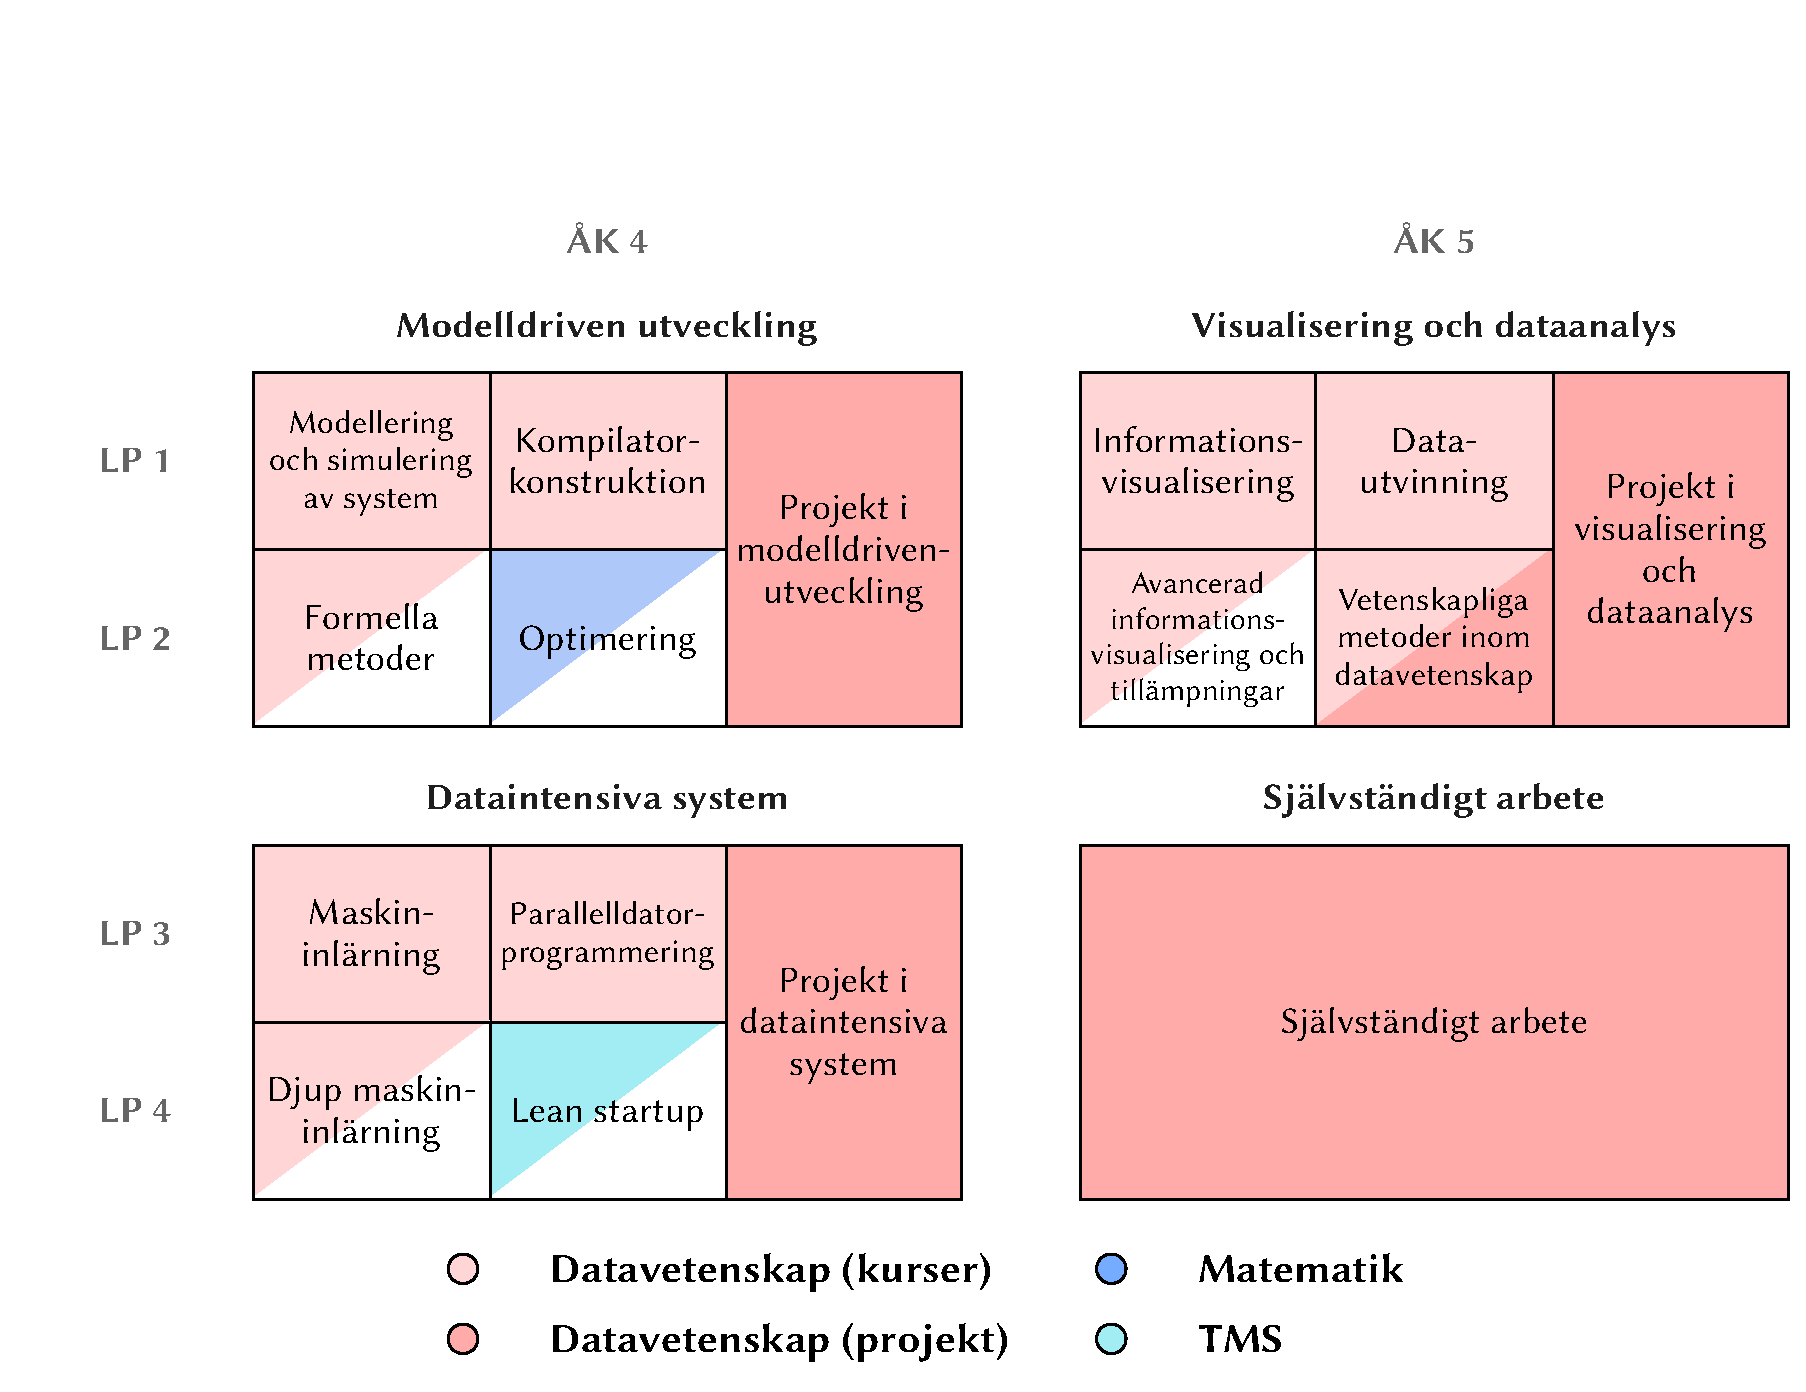
\includegraphics[width=\columnwidth]{images/bs45.eps}
\caption{Upplägg årskurs 4--5. Termin 7--9 består vardera av fyra kurser och ett projekt och termin 10 består av ett självständigt arbete.\label{fig:bs45}}
\end{figure}

Årskurs 4 och 5 ger en fördjupning i karaktärsämnen och yrkesrollen. Figur~\ref{fig:bs45} beskriver innehåll och progression under årskurs 4 och 5. Under termin 7–9 läser studenterna fyra kurser (5 hp vardera) och ett projekt (10 hp) varje termin. De fyra kurserna ger en teoretisk fördjupning och projektet, som täcker hela CDIO-cykeln, ger praktiska färdigheter och fördjupning inom yrkesrollen. Det ger även studenterna möjlighet att snabbt omsätta de mera teoretiska kunskaperna och frågeställningarna från kurserna inom exempelvis etik eller mjukvarans roll i samhället i ett praktiskt projekt. Under termin 10 genomför studenterna ett självständigt arbete som omfattar 30 hp. Termin 7–9 kommer att ha terminskoordinatorer som ansvarar för att skapa ett sammanhang mellan kurser och projekt. Terminskoordinatorn kommer att vara en senior forskare från aktuellt fördjupningsområde som tillsammans med en expert på projekt och projektmetodik ansvarar för terminens projekt.

Varje termin har ett fördjupningsområde inom det övergripande temat modellens roll i mjukvaruutveckling och ger något eller några perspektiv på hur modeller används. De tre fördjupningsområdena är starkt kopplade till forskning inom datavetenskap. Den forskargrupp som står närmast ett område ansvarar för projektet och en majoritet av kurserna.

Termin 7, \emph{Modellbaserad utveckling}, fokuserar på hur modeller kan användas för att utveckla eller testa egenskaper hos system. Terminen börjar med kurserna \emph{Modellering och simulering av system} och \emph{Kompilatorkonstruktion}. Den första av dessa två diskuterar hur man kan modellera och simulera ett system för att exempelvis testa egenskaper hos systemet innan implementationen i något programspråk påbörjas. Den senare kursen fokuserar på datorspråk och översättningar mellan dessa och belyser hur modellbeskrivningsspråk kan översättas till programspråkskod eller exekverbar kod. Under projektkursen kommer studenterna att tillämpa modellbaserad utveckling för att lösa ett öppet problem i en realistisk miljö, medan kurserna belyser den teori och de algoritmer som exempelvis de verktyg som används bygger på. Studenterna får i kurserna implementera enklare versioner av verktygen och i projektet använda verktyg som används i yrkeslivet. Terminen avslutas med kurserna \emph{Formella metoder} och \emph{Optimering} som fokuserar på hur egenskaper hos en modell kan formellt verifieras samt hur modeller kan optimeras.

Termin 8, \emph{Dataintensiva system}, fokuserar på hur modeller kan utvinnas och läras ur data. Terminen inleds med kurserna \emph{Maskininlärning} och \emph{Parallelldatorprogrammering}. I den första introduceras algoritmer för maskininlärning för att analysera och identifiera information i stora datamängder. I den senare ges en insikt i hur stora beräkningar kan utföras mer effektivt genom parallellbearbetning och vilka typer av utmaningar detta kan medföra. Projektkursen ger studenterna praktiska erfarenheter koppade till modellering och tillämpning av algoritmer för maskininlärning. Kursen \emph{Djup maskininlärning} är en fortsättningskurs som belyser aspekter som kräver viss erfarenhet såsom hur man utvärderar resultat, hur mycket data som behövs, eller när olika algoritmer är tillämpliga, vilket studenterna får i det pågående projektet.

Termin 9, \emph{Visualisering och dataanalys} fokuserar på visualisering och hur modeller kan kommuniceras till människor för vidare, fördjupad, analys. De två första kurserna \emph{Informationsvisualisering} och \emph{Datautvinning} ger grunderna i hur man visualiserar information samt hur man utvinner data ur ostrukturerade källor. Kurserna ger tillsammans den grundläggande förståelse som behövs i projektet som handlar om analys med stöd av visualiseringar, ett arbetssätt där människan med hjälp av avancerade flexibla visualiseringar försöker förstå komplexa modeller och den information som dessa innehåller. Kursen \emph{Avancerad informationsvisualisering} och tillämpningar bygger vidare på de inledande kurserna och på projektkursen och belyser hur visualisering tillämpas inom exempelvis bioinformation och geografi.

De tre projekten i termin 7–-9 ger förutom en möjlighet att tillämpa kunskaper från de olika fördjupningsområdena, även en progression i yrkesrollen och att arbeta i projekt. Det första av de tre projekten ger studenterna möjlighet att mera självständigt pröva några av de olika metoder och aktiviteter inom agila utvecklingsprocesser som introducerades i kursen \emph{Mjukvaruutvecklingsprojekt} i årskurs 2. I det andra projektet läggs fokus på att göra ett utvecklingsteam så effektivt som möjligt, genom att införa så kallade Lean agile-metoder. Här låter man studenterna arbeta under former som påminner om en startup, där tid och resurser är begränsade. I den tredje projektkursen skall studenterna självständigt genomföra ett agilt projekt.

Termin 10 består av ett självständigt arbete som avslutar och sammanfattar utbildningen. För att förbereda inför detta ges en fördjupning i \emph{Vetenskapliga metoder inom datavetenskap} i termin 9. Det är en seminariekurs där studenter läser, presenterar och diskuterar/opponerar på vetenskapliga artiklar, med fokus på vetenskapliga frågeställningar och metod. Studenterna väljer, i samråd med forskare från de olika fördjupningsområdena, lämpliga artiklar att läsa. En stor del av kursens examination är att ta fram ett planeringsdokument med frågeställningar och metod för det självständiga arbetet.

\subsection{Utbildningens vetenskapliga grund och forskningsanknytning}

 CDIO-konceptet används för att säkra att det föreslagna utbildningsprogrammet uppnår en hög nivå av ingenjörsmässighet. Det kan vara svårt att tydligt skilja vetenskap och ingenjörskonst, särskilt inom tillämpade vetenskaper. Det finns tillämpad forskning och grundläggande ingenjörskonst. Det är inte självklart att den ena står närmare forskning och vetenskap än den andra. De två likställs därför under programmets inledning och tidiga kurser fokuserar på att ta fram tekniska lösningar till komplexa problem och verifiera dessa lösningar samtidigt som ett helhetsperspektiv krävs. På liknande sätt övar bland annat kurserna \emph{Databaser och datamodellering} och \emph{Objektorienterad programmering} studenterna i att värdera och prioritera olika lösningar till ett problem, samt argumentera för dessa. Kursen \emph{Tillämpad sannolikhetslära och statistik} i slutet av årskurs 1 täcker hypoteser, experiment och hypotesprövning, som sedan kommer att tillämpas i kommande kurser.

I årskurs 3 ger kursen \emph{Vetenskapliga metoder} en introduktion till metodik och hur man genomför en vetenskaplig studie. Kursen belyser kopplingen till ingenjörsmässighet samt samspelet mellan vetenskap och ingenjörskonst. I det självständiga arbetet i slutet av årskurs 3 ska studenterna självständigt formulera ett problem i samråd med en handledare och en lösning till detta, samt påvisa att det är en lösning. De skall använda ingenjörsmässiga och/eller vetenskapliga metoder för det. Innan studenterna får lägga fram sitt självständiga arbete skall de ha auskulterat på tre andra framläggningar, på minst samma nivå. För att förbereda dem inför det egna självständiga arbetet uppmanas studenterna från och med termin 4 att börja auskultera på andra arbeten, främst på kandidatnivå. Det kan också göras vid arbeten på högre nivå till exempel masters, licentiat eller doktor. Studenterna skall även auskultera på tre arbeten på mastersnivå eller högre inför det självständiga arbetet i termin 10 och de kommer att uppmuntras göra detta från och med termin 6.

I årskurs 4 och 5 kopplas i princip samtliga kurser till den forskning som bedrivs inom Institutionen för datavetenskap och medieteknik såsom dataintensiv mjukvaruteknik och informationsvisualisering. Kurserna och projekten kommer under dessa årskurser att ha en väldigt tydlig anknytning till aktuell forskning och forskningsresultat. Många av de metoder och verktyg, samt den plattform som används för laborationer, kommer direkt från eller används inom forskningen vid institutionen.

Under årskurs 4 och 5 kommer en stor del av kurslitteraturen att bestå av vetenskapliga artiklar, men redan under årskurs 1 kommer vissa kurser att använda vetenskapliga artiklar som komplement till kurslitteraturen. Ett exempel på en sådan artikel är E.F. Codds ``A Relational Model of Data for Large Shared Data Banks'' från 1970 som introducerar relationsmodellen som fortfarande är den dominerande modellen för databaser. Syftet med artiklarna som används på kurserna under årskurs 1 är främst att öva studenterna på att söka efter och läsa vetenskapliga artiklar, samt påminna om att stora idéer ofta börjar som vetenskapliga resultat i artiklar. Under årskurs 2 och 3 ökar antalet kurser som använder vetenskapliga artiklar som komplement och syftet med artiklarna breddas till att också vara ett innehållsmässigt komplement till kurslitteraturen.

I kursen \emph{Teknisk kommunikation} i årskurs 2 undervisas i hur man söker efter information och artiklar, hur man läser en artikel, samt hur man analyserar och bedömer en artikels innehåll. I kursen \emph{Introducerade projekt} i årskurs 1 skall studenterna söka efter information för att lösa problem, men detta rör sig främst om teknisk information som snabbt kan utvärderas. Efter undervisning i hur man söker och analyserar artiklar kommer kurserna att ställa större krav på att självständigt söka information och ta ställning till denna. Denna färdighet byggs vidare på i kursen \emph{Vetenskapliga metoder}, där studenterna undervisas i att värdera metoder och hur dessa påverkar vilka frågor som kan besvaras samt hur tillförlitligt och generaliserbart resultatet är. Det självständiga arbetet i slutet av årskurs 3 är den första kursen där studenterna själva ska välja all litteratur (i samråd med handledare). I årskurs 4 och 5 skall studenterna självständigt söka efter och välja kompletterande litteratur i de flesta av kurserna, i synnerhet projektkurserna.

Under årskurs 1–3 kommer den programansvarige att ha det operativa ansvaret för att det finns forskningsanknytning och ett forskande perspektiv i utbildningen. Under termin 7–9 flyttas detta ansvar till terminskoordinatorerna, som är experter inom det området som fördjupningen berör. Under termin 10 delas det operativa ansvaret mellan handledarna och examinatorerna för de självständiga arbetena.

\section{Motivering för ansökan om examensrättigheter}

Linnéuniversitetet söker rättigheter att examinera civilingenjörer i mjukvaruteknik av tre skäl. Nedan följer bakgrund till, analys av och motivering för dessa.

\begin{itemize}
	\item Industrin, både i regionen och nationellt, har ett stort behov av att rekrytera kvalificerad arbetskraft och efterfrågar särskilt civilingenjörer inom data och informationsteknik.
	\item Linnéuniversitetet har en stark tradition av yrkesutbildning och strävar mot ett brett erbjudande med hög kvalitet. Universitetet har därför arbetat strategiskt för att utöka sitt erbjudande med en examensrättighet för civilingenjörer.
	\item Fakulteten för teknik vill erbjuda en spetsutbildning med högre grad av ingenjörsmässighet och yrkeslivskoppling inom datavetenskap.
\end{itemize}

Den regionala industrin har under flera år efterlyst en regional civilingenjörsutbildning inom data och informationsteknik då de upplever att det är väldigt svårt att rekrytera personer med civilingenjörsutbildning till regionen. Flera anger att de har slutat att försöka och överväger alternativa lösningar som att omlokalisera delar av eller hela sin verksamhet. Många företag och kommunerna i regionen anser att den föreslagna civilingenjörsutbildningen är avgörande för en fortsatt tillväxt i regionen och, i ett längre perspektiv, vissa verksamheters långsiktiga överlevnad. Till ansökan bifogas stödbrev och avsiktsförklaringar från industri och organisationer i regionen (Växjö och Kalmar) i appendix~\ref{app:stodbrev}. Stödbrev för att belysa deras behov och intresse av en civilingenjörsutbildning i regionen.

Att förse regionen och landet med kompetent arbetskraft är en av universitetets främsta uppgifter och därför framhålls detta som den främsta anledningen till att Linnéuniversitetet söker examensrättigheter. Den föreslagna utbildningen är dock inte avsedd som en regional utbildning utan är byggd för att motsvara det nationella behov som anges i avsnitt~\ref{sec:analysindbehov} och studenter kommer efter examen att kunna söka sig regionalt, nationellt och internationellt. Erfarenhet från befintliga längre yrkesutbildningar visar dock att några studenter antingen söker sig till utbildningen för att de inte vill lämna regionen eller under sin studietid rotar sig i regionen och således stannar kvar efter examen. Det stora inslaget av projekt som utförs tillsammans med näringslivet kommer troligtvis att leda till att studenter rekryteras av företag i regionen. Det här resonemanget stöds av en rapport från Teknikföretagen\footfullcite{teknikforetagen} som menar att det bästa sättet att rekytera utanför storstadsregionerna är att samarbeta med universitet och högskolor i regionen (se avsnitt~\ref{sec:analysindbehov}).

Nästa skäl till ansökan av examensrättigheter är att Linnéuniversitetet har en lång tradition av yrkesutbildningar, exempelvis högskoleingenjör och lärare. Samtidigt är universitetet idag ett av få svenska lärosäten som inte har rättigheter att examinera civilingenjörer. Då detta är en efterfrågad examen av både industri och studenter är det av strategisk vikt att erhålla rättigheter att erbjuda denna examen, för att säkerställa möjligheter att rekrytera studenter inom teknikområden i framtiden. Linnéuniversitetet tappar redan studenter som vill läsa vidare mot en civilingenjörsexamen efter sin högskoleingenjörsexamen, då en masterexamen inte uppfattas ha samma värde som en civilingenjörsexamen. Baserat på det söktryck och intresse som finns för de befintliga civilingenjörsutbildningarna inom data och informationsteknik (se avsnitt~\ref{sec:analysbefintnat}) anser Linnéuniversitetet att det finns utrymme för flera utbildningar.

De två skäl som anges ovan är viktiga, men de kräver att en utbildning av hög kvalitet kan erbjudas. Så, det sista skälet till att Linnéuniversitetet söker rättigheter är att det kan erbjuda en högkvalitativ utbildning som tillför något utöver det som erbjuds av de befintliga civilingenjörsutbildningarna inom data och informationsteknik. Det utbildningsprogram som föreslås i ansökan började som ett initiativ att göra det befintliga mastersprogrammet i mjukvaruteknik mera anpassat mot yrkeslivets behov, genom att bland annat öka inslag av projekt och ingenjörsmässighet. Samtidigt har programmets starka koppling mot forskning bibehållits. Arbetet resulterade bland annat i upplägget med tre korta fördjupningar med både en teoretisk och en praktisk fördjupning. Arbetet med att förändra mastersprogrammet finansierades av KK-stiftelsen\footnote{``Nyutveckling av masterprogrammet i datavetenskap'', KK-stiftelsen Dnr: 20150316} och skedde i samarbete med näringslivet i regionen (Kronoberg, Kalmar och Blekinge), exempelvis Combitech och IKEA. När årskurs 4 och 5 var klara skapades innehållet i årskurs 1–3 för att på bästa möjliga sätt förbereda studenterna. Det finns en tydlig progression genom programmet, där studenternas kunskaper, färdigheter och perspektiv inom och på datavetenskap, matematik, ingenjörsmässighet och vetenskaplighet utvecklas. Den stora andelen projektkurser kommer att förbereda studenterna för yrkeslivet, i linje med vad IT\&Telekombolagen\footfullcite{ittelekom} föreslår för att förbättra arbetslivsförberedelserna inom utbildningen.

\section{Analys av behov i ett regionalt och nationellt perspektiv}\label{sec:analysindbehov}

Teknikföretagen, IT\&Telekomföretagen och Swedsoft\footfullcite{swedsoft} har i slutet av 2017 och under inledningen av 2018 publicerat rapporter som kartlägger kompetensbehov inom data och informationsteknik i svensk industri. Man är överens om att mjukvara får en allt större roll i samhället och ekonomin. Dessutom finns det ett stort rekryteringsbehov av ingenjörer med mjukvaruspecialisering. Samtidigt visar rapporterna på att detta är en av de mest bekymmersamma kompetenserna att rekrytera; IT\&Telekombolagen benämner kompetensbristen inom IT-sektorn ``en av vår tids största utmaningar''.

Enligt Statistiska centralbyråns arbetskraftsbarometer för 2017 bedömer 8 av 10 arbetsgivare att de kommer att öka antalet anställda med civilingenjörsutbildning inom datateknik till 2020\footfullcite{barometern17}. Samtidigt bedömer mer än 60~\% av tillfrågade arbetsgivare att det finns en brist på nyutexaminerade och mer än 80~\% anser att det finns en brist på yrkeserfarna. I samma undersökning rapporteras en ännu större brist av programmerare och systemvetare; här anser nästan 80~\% av arbetsgivarna att det råder brist. Så även om civilingenjörsprognosen innefattar elektronik och automation är det rimligt att använda den för att dra slutsatser för datateknik och datavetenskap.

Swedsofts rapport menar att heterogeniteten i gruppen mjukvaruutvecklare medför att kompentenserna som krävs varierar från företag till företag. Den absolut viktigaste kompetensen är generell programmeringskompetens följd av specifik systemnära programmering. Viktiga kompletterande kompetenser som söks är bland annat system- och systemarkitekturkompetens och matematisk kompetens, medan kunskap inom ekonomi och affärsverksamhet anses minst viktigt av de som undersöks. Bland de viktiga kompletterande förmågor som söks står tre ut: logiskt analytisk förmåga (cirka 90~\% anser denna avgörande), kreativ och innovativ (cirka 80~\%), samt självledarskap och självkännedom (cirka 80~\%). Förmågor såsom ledarskap anses mindre avgörande (cirka 45~\%). Djupintervjuer med deltagare belyser särskilt behovet av samarbete mellan mjukvaruutvecklare och personer med andra kompetenser, exempelvis nämns fysiker och mekaniker som viktiga för automation och robotar.

Precis som i rapporten från Swedsoft menar IT\&Telekombolagen att generell programmeringskompetens är viktigare än specifik kunskap i ett särskilt språk. De efterlyser också bättre arbetslivsförberedelser från högskoleutbildningar genom fortlöpande färdighetsträning och arbetslivskontakter under utbildningstiden. De föreslår specifikt att det skall finnas två obligatoriska kursmoment i aktivt samarbete med tänkbara framtida arbetsgivare. De menar vidare att en sådan ansats även kan hjälpa till att öka kompetensen hos de arbetsgivare som medverkar i dessa moment, så att det blir en dubbelriktad satsning.

\section{Analys av befintligt regionalt och nationellt utbildningsutbud}\label{sec:analysbefintnat}

Hösten 2017 erbjöds det totalt 19 civilingenjörsutbildningar inom data och informationsvetenskap vid 13 lärosäten. En stor del av dessa har generella benämningar såsom Datateknik, Informationsteknik och Mjukvaruteknik. Innehållet i de flesta av programmen kan beskrivas som en kombination av, i ACM:s nomenklatur, Computer Science, Software Engineering och Computer Engineering. Majoriteten av programmen bedöms ha ett huvudsakligt fokus på datavetenskap (Computer Science). Programmen i Datorsäkerhet, Spel- och programvaruteknik och Robotik har mera specifika namn och i stor utsträckning även specifikt innehåll.

Den föreslagna utbildningen i mjukvaruteknik är en kombination av datavetenskap och mjukvaruteknik. Baserat på en analys av utbildningsplaner ligger den föreslagna utbildningen närmast de program som benämns Informationsteknik eller Mjukvaruteknik vid Linköping tekniska högskola, Chalmers tekniska högskola och Kungliga tekniska högskolan. Den föreslagna utbildningen skiljer sig dock från dessa på några punkter, bland annat det stora inslaget av projekt och de tre obligatoriska fördjupningsområdena. Programmet i Spel- och programvaruteknik vid Blekinge Tekniska Högskola har ett stort inslag av projekt och programvaruutveckling, men skiljer sig samtidigt då det har en fokus på datorspelsteknik.

Söktrycket för civilingenjörsutbildningar inom området är högt. Enligt UKÄ:s sök- och antagningsstatistik från 2016 och 2017 finns det fler sökande än platser. De olika programmen hade 2017 totalt nästan 14 000 sökande och nästan 2 400 förstahandssökande. De existerande program som mest liknar den föreslagna utbildningen hade totalt cirka 2 200 sökande, 640 förstahandssökande och 530 antagna.

Antalet sökande varierar stort mellan etablerade civilingenjörsutbildningar vid exempelvis Chalmers tekniska högskola och Kungliga tekniska högskolan och de nyare vid exempelvis Karlstads universitet och Örebro universitet. Det är dock endast en utbildning som 2017 inte hade några reserver, vilket tyder på att även de nyare utbildningarna fyller sina platser. Tidigare statistik visar dock på att det har tagit tid för de nyare utbildningarna att nå upp till dessa sök- och antagningstal.


\section{Analys av befintliga utbildningar inom data och informationsteknik vid Linnéuniversitetet}\label{sec:analysbefintlnu}

Linnéuniversitetet erbjuder ett högskoleexamensprogram, tre kandidatprogram, två högskoleingenjörsprogram, ett magisterprogram och ett mastersprogram inom datavetenskap och datateknik. Se tabell~\ref{tab:dvprogram} för en översikt. Utöver dessa erbjuds även utbildningar inom medieteknik och informatik på grund och avancerad nivå. De senare skiljer sig dock avsevärt från den föreslagna utbildningen och diskuteras därför inte.

\begin{table}
\centering
\caption{Utbildningsprogram inom datavetenskap och datateknik vid Linnéuniversitetet. Antagna anger det antal studenter som antogs inför läsåret 2017/2018.\label{tab:dvprogram}}
%\resizebox{\columnwidth}{!}{%
\begin{threeparttable}
\begin{tabular}{p{5cm}lrr}
\toprule
\textbf{\textsf{Namn}} & \textbf{\textsf{Examen}} & \textbf{\textsf{Hp}} & \textbf{\textsf{Antagna}}\tabularnewline
\midrule
Webbprogrammerare & Högskoleexamen & 120 & 125\tabularnewline
Datateknik & Högskoleingenjörsexamen & 180 & 39\tabularnewline
Mjukvaruteknik\tnote{1} & Högskoleingenjörsexamen & & \tabularnewline
Programvaruteknik & Kandidatexamen & 180 & 93\tabularnewline
Nätverkssäkerhet & Kandidatexamen & 180 & 64\tabularnewline
Utveckling och drift av mjukvarusystem & Kandidatexamen & 180 & 130\tabularnewline
Programvaruteknik & Magisterexamen & 60 & 24\tabularnewline
Programvaruteknik & Masterexamen & 120 & 23\tabularnewline
\bottomrule
\end{tabular}
\begin{tablenotes}
\item[1] Från och med läsåret 2018/2019.
\end{tablenotes}\end{threeparttable}
\end{table}

De befintliga utbildningarna på grundnivå täcker olika delar av datavetenskap och datateknik. Högskoleingenjörsprogrammet i datateknik täcker områdena mellan mjukvara och hårdvara och fokuserar i huvudsak på inbyggda system. Kandidatprogrammet i programvaruteknik är en traditionell datavetenskaplig utbildning med fokus på mjukvaruutveckling, medan kandidatprogrammen i \emph{Nätverkssäkerhet} och \emph{Utveckling och drift av mjukvarusystem} har en datavetenskaplig kärna men ett starkt fokus på tillämpningsområden. Nätverkssäkerhet fokuserar på datorsäkerhet med avseende på både mjukvara och datornät och innehåller bland annat kurser i kryptering och administration av nätverk. Utveckling och drift av mjukvarusystem fokuserar på området mellan mjukvaruutveckling och systemdrift, så kallade Development Operations (DevOps) och innehåller bland annat kurser i systemadministration, kontinuerlig leverans av mjukvara och konfigurationshantering. Högskoleprogrammet i webbprogrammering är en yrkesförberedande utbildning som fokuserar på utveckling av mjukvara för webben exempelvis webbplatser och backend-system.

I ansökningsomgången 2017 sökte totalt cirka 3 400 studenter, varav 587 förhandssökande, till våra fem utbildningar på grundnivå. De två mest populära programmen, \emph{Webbprogrammerare} och \emph{Utveckling och drift av mjukvarusystem} stod för över 70~\% av det totala söktrycket. Av de sökande antogs 428 och 313 registrerades.

Det föreslagna civilingenjörsprogrammet är innehållsmässigt mest likt \emph{Högskoleingenjörsprogrammet i datateknik} och \emph{Kandidatprogrammet i programvaruteknik}. Dessa hade totalt 518 sökande (99 i första hand) i ansökningsomgången 2017, varav 132 antogs och 98 registrerades.

Utbildningsutbudet inom datavetenskap vid Linnéuniversitetet ses kontinuerligt över och förändras efter behov. Inför läsåret 2018/2019 kommer exempelvis ett nytt högskoleingenjörsprogram i mjukvaruteknik startas i Kalmar och inför läsåret 2019/2020 kommer de befintliga utbildningarna på avancerad nivå förändras så att de tydligare följer det upplägg som föreslås för civilingenjörsprogrammet. Det möjliggör samläsning och medför ett större utbud av valbara kurser för den föreslagna utbildningen. Om rättigheter att examinera civilingenjörer erhålls kommer hänsyn att tas till detta vid framtida utbildningsöversyn.
